%%%%%%%%%%%%%%%%%%%%%%%%%%%%%%%%%%%%%%%%%%%%%%%%%%%%%%%%%%%%%%%%%%%%%%%%%%%%%%%%
% main.tex
%
% $Id: main.tex 1036 2016-02-02 05:28:24Z hayashi $
%
%%%%%%%%%%%%%%%%%%%%%%%%%%%%%%%%%%%%%%%%%%%%%%%%%%%%%%%%%%%%%%%%%%%%%%%%%%%%%%%%

\documentclass[a4paper, 10pt]{jbook} % 通常の文書

%%%%%%%%%%%%%%%%%%%%%%%%%%%%%%%%%%%%%%%%%%%%%%%%%%%%%%%%%%%%%%%%%%%%%%%%%%%%%%%%
%%% PREAMBLE
%%%%%%%%%%%%%%%%%%%%%%%%%%%%%%%%%%%%%%%%%%%%%%%%%%%%%%%%%%%%%%%%%%%%%%%%%%%%%%%%

%% Packages
%\usepackage{amsfonts}
\usepackage[cmex10]{amsmath}
\usepackage{bm}
\usepackage{booktabs}
%\usepackage{enumitem}
\usepackage[dvipdfmx]{graphicx}
\usepackage{listings}
%\usepackage{longtable}
%\usepackage{multirow}

%% Path to eps files(use with package graphicx)
\graphicspath{{./psfiles/}}

%% Option of lstset(listings)
%\lstset{
%	language = c,
%	numbers = left,
%	stepnumber = 1,
%	numberstyle = \itshape,
%	numbersep = 10pt,
%	breaklines = true,
%	breakindent = 20pt,
%	frame = single,
%	framesep = 3pt,
%	basicstyle = \ttfamily,
%	commentstyle = \ttfamily,
%	keywordstyle = \ttfamily,
%}

%% make a booklet of pdf
\usepackage[
	dvipdfmx,
	bookmarks=true,
	bookmarksnumbered=true,
	bookmarkstype=toc,
	colorlinks=true,
	linkcolor=black,
	citecolor=black,
	filecolor=black,
	setpagesize=false,
%	pagecolor=black,
	urlcolor=black
]{hyperref}

%% translate the letter code of booklet from EUC to Unicode
\ifnum 42146=\euc"A4A2 \AtBeginDvi{\special{pdf:tounicode EUC-UCS2}}\else
\AtBeginDvi{\special{pdf:tounicode 90ms-RKSJ-UCS2}}\fi
%% add section number to equation number
%\makeatletter
%    \renewcommand{\theequation}{
%	    \thesection.\arabic{equation}
%	}
%    \@addtoreset{equation}{section}
%\makeatother


%%%%%%%%%%%%%%%%%%%%%%%%%%%%%%%%%%%%%%%%%%%%%%%%%%%%%%%%%%%%%%%%%%%%%%%%%%%%%%%%
%%% TITLE, AUTHOR, DATE
%%%%%%%%%%%%%%%%%%%%%%%%%%%%%%%%%%%%%%%%%%%%%%%%%%%%%%%%%%%%%%%%%%%%%%%%%%%%%%%%

%% Title
\title{
	AzLib の手引き書
}

%% Author
\author{
	hayashi@azlab
}

%% Date
\date{
	最終更新日:\today
}


%%%%%%%%%%%%%%%%%%%%%%%%%%%%%%%%%%%%%%%%%%%%%%%%%%%%%%%%%%%%%%%%%%%%%%%%%%%%%%%%
%%% BODY
%%%%%%%%%%%%%%%%%%%%%%%%%%%%%%%%%%%%%%%%%%%%%%%%%%%%%%%%%%%%%%%%%%%%%%%%%%%%%%%%

\begin{document}
\maketitle

%\begin{abstract}
%本書は,名古屋大学畔上研究室内の開発環境であるAzLib(アズリブ)の手引き書です.
%AzLibを利用する人の手助けをすることを目的として書かれています.
%第\ref{sec:abstract}章で概要を説明し,第\ref{sec:base}章以降で詳細を説明します.
%細かい部分はソースコードを読むのが一番だと思うので,本書ではソースコードを
%書くことは極力しません.
%\end{abstract}

\tableofcontents
%\listoffigures
%\listoftables
\newpage

\chapter{概要} \label{chap:abstract}
この章では,AzLibの概要を説明します.
ご存知のように,畔上研究室では最適化の理論と計算方法の開発を行っています.
AzLibは,それらを実行するプログラムの開発環境です.
Subversionの中のazlibというディレクトリが本体となります.

% 解析例
「百聞は一見に如かず」なので,AzLibで開発したプログラムによる簡単な最適化の例を
見てみましょう.
図\ref{fg:analysis_eg_init}は,左端の面が固定されている片持ち梁の有限要素モデル
です.
\begin{figure}
	\centering 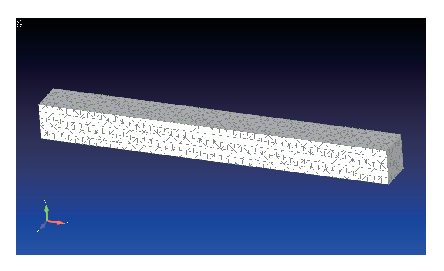
\includegraphics{analysis_eg_init.eps}
	\caption{形状最適化前のモデル} \label{fg:analysis_eg_init}
\end{figure}
今回は概要なので,細かい設定の説明は省きます.
このモデルの右端に鉛直下向きの力を加えたとき,体積制約付きで剛性を最大化する
という形状最適化問題を考えます.
図\ref{fg:analysis_eg_result}は,AzLibを使ってこの最適化問題を解いたときの
最適形状です.
\begin{figure}
	\centering 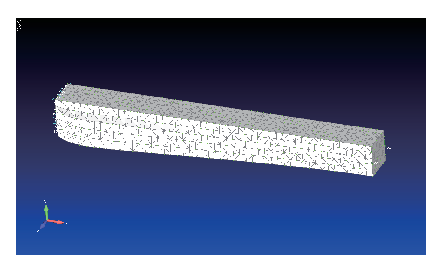
\includegraphics{analysis_eg_result.eps}
	\caption{形状最適化後のモデル} \label{fg:analysis_eg_result}
\end{figure}
このような最適化を行うプログラムを開発する際の土台となるのがAzLibということに
なります.

% 章の役割
畔上研究室の理論では,最適化の実装に有限要素法を用いています.
有限要素法には,行列演算をはじめとする数多くの数値計算が用いられます.
また,あらゆる処理に対してエラーが発生したときの対応もしなければなりません.
さらに,有限要素法は要素の情報の格納に膨大なメモリを必要とするので,使用する
メモリを適切に管理しなければなりません.
最適化の実装にあたって,多くの要件を満たさなければならないのです.
そのため,プログラムを役割ごとにいくつかのディレクトリに分けて,見通しをよく
しています.

まず,\ref{sec:abstract_directory}節ではそれぞれのディレクトリの役割について
説明します. 
次に,\ref{sec:abstract_usage}節ではAzLibの利用法について説明します. 
最後に,\ref{sec:abstract_develop}節ではAzLibの開発方法について説明します.

\section{各ディレクトリの概要} \label{sec:abstract_directory}
ここでは,AzLibを構成するディレクトリの概要を説明します.

AzLibのソースコードの本体はSubversion/azlib/trunk/srcにあります.
実際に見てみると,次の $5$ つのディレクトリがあります.
\begin{itemize}
	\item base
	\item fem
	\item gui
	\item image
	\item mathematics
\end{itemize}

baseディレクトリには,あらゆる処理の土台(base)となるソースコードが含まれて
います.
たとえば,不適切な処理を行わないようにするエラーチェックの仕組みや,使用する
メモリの管理を行う仕組みなどが実装されています.

femディレクトリには,有限要素法の処理に関するソースコードが含まれています.

guiディレクトリには,(執筆中)

imageディレクトリには,(執筆中)

mathematicsディレクトリには,femディレクトリで用いる有限要素法の処理で必要と
なる数値計算に関するソースコードが含まれています.

以上 $5$ つのディレクトリには,図\ref{fg:abstract_hierarchy}のような階層構造が
あることがなんとなくわかると思います.
\begin{figure}
	\centering 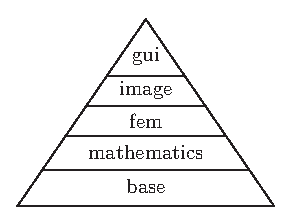
\includegraphics{abstract_hierarchy.eps}
	\caption{AzLibのディレクトリの階層構造} \label{fg:abstract_hierarchy}
\end{figure}
つまり,baseディレクトリのソースコードを土台にしてmathematicsディレクトリの
ソースコードが書かれており,mathematicsディレクトリのソースコードを土台にして
femディレクトリのソースコードが書かれており,・・・ということです.
第\ref{chap:base}章からはそれぞれのディレクトリの中身を説明しますが,
この階層構造で土台となるディレクトリから順に説明していくことにします.


\section{利用方法} \label{sec:abstract_usage}
ここでは,AzLibの使い方を説明します.

\ref{sec:abstract_directory}節で説明したそれぞれのディレクトリの中を見ると
わかりますが,ソースコードはすべてC言語で書かれています.
C言語については,Webで検索すればいくらでも情報が得られます.
そのため,本書ではC言語の基礎についての説明を省きます.

また,コンパイルはすべてmakefileを利用して行います.
makefileについてもWebで情報が得られるので,説明を省きます.
よくわからなければ,わかっている人に聞きましょう.
gccを用いてコンパイルするので,dnfでインストールしておいてください.

\subsection{基本的な使い方}
最適化の手続き本体は,main関数の中で記述することになります.
ここでは例を通して,AzLibを使って最適化を行うプログラムのソースコードを
眺めながら,実際にコンパイルしてみましょう.
今回は,Linuxの端末上でコンパイルすることを前提として説明します.

本章のはじめに簡単な最適化の例を見ましたが,この最適化のソースコードは
Subversion/azlib/trunk/examples/trac\_methodにあります.
まずは端末を開いてこのディレクトリまで移動し,エディタで最適化を行う
プログラムのソースコードを開いてみましょう.
\begin{verbatim}
    $ cd ~/Subversion/azlib/trunk/examples/trac_method
    $ vim trac_method.c
\end{verbatim}
この例ではエディタとしてvimを使っていますが,好きなものを使ってください.

$5$ 行目から $7$ 行目で,AzLibのbaseディレクトリ,mathematicsディレクトリ,
femディレクトリのヘッダファイルを読み込んでいます.
そこからしばらくは,このソースコードで独自に定義しているマクロや構造体,関数の
プロトタイプ宣言が続きます.
そして $69$ 行目から,main関数で最適化の手続きを記述しています.
以降ではプログラムにおける最適化の流れを確認し,実際に実行してみます.

\subsection{最適化の手続き}
main関数の中を簡単に説明します.
最適化の解析は,有限要素法を用いて行います.
はじめに解析するモデルの要素や節点などのデータを読み込み,最適化の
アルゴリズムを実行して,最後に最適化後のモデルのデータを出力します.

要素や節点などのデータは独自の構造体で管理します.
たとえば,$73$ 行目の\texttt{NODE\_ARRAY}型変数\texttt{node}で節点のデータを,
$74$ 行目の\texttt{ELEMENT\_ARRAY}型変数\texttt{element}で要素のデータを
管理します.
この他にも,有限要素法に関係のあるデータのほとんどが構造体で管理されます.
詳しくは,\ref{chap:fem}章で説明します. % そのうち節番号に変更する

$94$ 行目では,ログの出力の量を調節する「ログ出力レベル」の設定をしています.
続く $97$,$98$,$99$ 行目では,そのログの出力先を設定しています.
ログ出力の詳細については,\ref{sec:log-output-utl}節で説明します.

ここで,ログ出力レベルの設定に使っている関数の呼び出し方を見てみましょう.
AzLibには,RC型と呼ばれる独自の変数の型があります.
main関数でRC型の関数を用いるときは,このように「\texttt{RC\_TRY\_MAIN}」
マクロを利用します.
RC型の詳細については,\ref{subsec:RC-type}節で説明します.

$102$ 行目では,解析で使用するメモリの上限値を設定しています.
十分な量のメモリを確保して,以降の解析を行います.

$105$ 行目から $132$ 行目までは,解析に関するパラメータやモデルのデータを変数に
格納しています.
このあたりは,どのような最適化プログラムでも同様の記述になるはずです.

$135$ 行目から $144$ 行目で,解析結果を書き出すファイルを用意しています.
直後の最適化の処理には,場合によっては膨大な時間がかかります.
最適化の処理を実行した後で「結果をファイルに書き出せません」ということに
ならないよう,最適化の処理の前でこれらのファイルを用意します.

$146$ 行目から $149$ 行目で,最適化を実行します.
main関数の下にある\texttt{optimization()}という関数に,最適化の
アルゴリズムを記述しています.

$152$ 行目から $165$ 行目で,最適化したモデルを出力しています.

$169$ 行目で,$102$ 行目で動的確保したメモリを解放しています.

以上のような流れで,最適化を実行しています.
今回は線形弾性体の形状最適化を行うプログラムの例でしたが,どのような
最適化でもmain関数の中は同様になると考えられるので,プログラムを書くときには
参考になると思います.

\subsection{最適化プログラムのコンパイル}
最後に,このソースコードのコンパイルをしてみましょう.
このディレクトリにはmakefileがすでにあり,\verb|make|を実行するだけでコンパイルが
できるようになっています.
実際にコンパイルしてみましょう.
\begin{verbatim}
    $ make
\end{verbatim}

\verb|make|を実行するだけだとコンパイルの手順がややわかりづらいので,少しだけ
説明しておきます.
\verb|make|を実行すると,まず本体のソースコードのオブジェクトファイルを
生成します.
次に,AzLibの各ディレクトリごとのライブラリファイルを生成します.
このとき,各ディレクトリごとに用意されているmakefileを使います.
必要なライブラリファイルを生成したら,それらをリンクして実行モジュールを生成
します.
trac\_method内のmakefileは,この一連の手順を行うように記述されています.

どのようなソースコードを書いても,makefileの基本的な書き方はほとんど
変わりません.
自分でソースコードを書いた場合も,このmakefileをコピーしたものを少し書き換える
だけで済むはずです.

この例の最適化プログラムは,通常のC言語の実行ファイルと同じ方法で実行します.
ただしmain関数に渡す引数がいくつかあるので,実行するためのスクリプトがあります.
実際はこのスクリプトを実行すれば,ソースコードのコンパイルから実行ファイルの実行
までをすべて行ってくれます.
run.shというファイルが実行のスクリプトなので,実行してみましょう.
\begin{verbatim}
    $ ./run.sh
\end{verbatim}

形状更新などの履歴を適度に出力しながら最適化を行う様子がわかると思います.
このようなログを出力することも,プログラムに求められることのひとつです.
ログの出力の仕組みは,baseディレクトリで実装されています.


\section{開発方法} \label{sec:abstract_develop}
ここでは,AzLibの開発方法を説明します.

AzLibはSubversionによってソースコードを一元的に管理しています.
(執筆中)


\newpage
\chapter{base/} \label{chap:base}

本章では,AzLibの土台とも言えるbaseディレクトリについて説明します.
このディレクトリでは,AzLibで採用されている様々な開発技術を実装しています.
まずはじめに,実装されているそれらの機能について概要を説明します.
AzLibを利用するだけであれば,この概要にだけ目を通しておけば十分でしょう.
それから,それらの技術を実装している関数群の細かい使い方を説明します.


\section{実装している機能の概要}
AzLibが実装している機能は,以下のものがあります.
\begin{itemize}
	\item エラー処理機能
	\item ログ出力機能
	\item メモリ管理機能
\end{itemize}

エラー処理機能は,プログラムがこちらの意図しない動作をしそうなときに,そのことを
知らせて強制終了するように処理する機能です.
たとえば,なんらかの数値を $0$ で割るような計算をしそうになったら,実行を途中で
止めなければなりません.
管理下にないメモリにアクセスしそうになったときも,未然に止めなければなりません.

ログ出力機能は,実行したプログラムが具体的にどのような計算の過程を経て最後の
結果にたどり着いたのかを自動的に出力する機能です.
ログファイルに限らず,実行途中の段階でも端末上に実行の過程を表示することで,
計算がちゃんと行われているかを即座に知ることができます.

メモリ管理機能は,プログラムが利用するメモリ領域を管理する機能です.
第\ref{chap:abstract}章でも少し説明しましたが,最適化のプログラムは精度を上げる
ために膨大なメモリを必要とします.
いわゆる「メモリの動的確保」を的確に,無駄なく行わなければなりません.
そのために,まずはじめに使用するメモリの合計量を宣言して確保しておき,その中から
必要なメモリを利用して,最後にすべて解放するようにします.

それぞれの機能の簡単な使い方について,次の節から説明していきます.
いくつかの部分で,具体例としてAzLib内のソースコードを使います.


\section{エラー処理機能の使い方}
AzLibでは,\textbf{RC型}(アールシーがた)と呼ばれる独自の変数型を用いて,エラー
処理機能を実装しています.
ここでは,その簡単な使い方を説明します.

\subsection{RC型} \label{subsec:RC-type}
AzLibの関数の多くは,RC型で定義されています.
RCはReturn Codeの略で,その関数が正常に実行されたかどうかを返り値とします.
返り値の種類を表\ref{tb:rc_pattern}に示します.
\begin{table}
\caption{エラーの分類} \label{tb:rc_pattern}
\centering
\begin{tabular}{ll}
\toprule
エラーの種類 & RC \\
\midrule
エラーなし & \texttt{NORMAL\_RC} \\
途中で処理を終了させる場合など & \texttt{END\_RC} \\
switch文の失敗など & \texttt{IMPLEMENT\_ERROR\_RC} \\
ファイルの読み込みの失敗など & \texttt{READ\_ERROR\_RC} \\
ファイルの書き込みの失敗など & \texttt{WRITE\_ERROR\_RC} \\
変換の失敗など & \texttt{CONVERT\_ERROR\_RC} \\
ポインタが\texttt{NULL}値であるなど & \texttt{NULL\_ERROR\_RC} \\
配列の動的確保の失敗など & \texttt{ALLOC\_ERROR\_RC} \\
ファイルオープンの失敗など & \texttt{OPEN\_ERROR\_RC} \\
ファイルクローズの失敗など & \texttt{CLOSE\_ERROR\_RC} \\
探索の失敗など & \texttt{SEEK\_ERROR\_RC} \\
データのフラッシュの失敗など & \texttt{FLUSH\_ERROR\_RC} \\
関数の引数が不適切であるなど & \texttt{ARG\_ERROR\_RC} \\
数値計算の失敗など & \texttt{CAL\_ERROR\_RC} \\
データのオーバーフローなど & \texttt{OVERFLOW\_ERROR\_RC} \\
データのアンダーフローなど & \texttt{UNDERFLOW\_ERROR\_RC} \\
$0$ が入ってはいけないときなど & \texttt{ZERO\_ERROR\_RC} \\
負の値が入ってはいけないときなど & \texttt{NEGATIVE\_ERROR\_RC} \\
 & \texttt{SUBMIT\_ERROR\_RC} \\
 & \texttt{OVERRUN\_ERROR\_RC} \\
 & \texttt{IGNORE\_ERROR\_RC} \\
いずれにもあてはまらない場合など & \texttt{UNKNOWN\_ERROR\_RC} \\
エラーとも呼びがたい場合など? & \texttt{SPECIAL\_RC} \\
\bottomrule
\end{tabular}
\end{table}
数が多いので,眺める程度の理解で大丈夫です.
また,使い分けに関して厳密なルールはないので,適当に使い分ければ大丈夫です.
C言語ではvoid型以外の関数の返り値は $1$ つなので,他に値を返したい場合は
ポインタを使うことになります.

RC型の関数を呼ぶときは,専用のマクロを使います.
もしその関数が正常に実行されなかったことを表す値が返却されたときには,そのことを
表示し,その時点でプログラムを強制終了します.

\subsection{\texttt{RC\_TRY\_MAIN}マクロ}
main関数でRC型の関数を使うときは,\verb|RC_TRY_MAIN|マクロを用います.
たとえば,第\ref{chap:abstract}章で見た剛性最大化プログラムのソースコード
trac\_method.cを見てみましょう.
94行目の\verb|set_log_level()|で,ログの出力レベルを設定しています.
このとき,\verb|RC_TRY_MAIN|マクロを使って関数を呼んでいます.
そこから下でも,ログの出力先の設定や使用するメモリの上限値の設定など,数多くの
処理を行う関数がRC型で定義されており,\verb|RC_TRY_MAIN|マクロを使って実行して
います.

\subsection{\texttt{RC\_TRY}マクロ}
main関数以外の関数でRC型の関数を使うときは,\verb|RC_TRY|マクロを用います.
たとえば,mathematicsディレクトリのlu.cを見てみましょう.
25行目から,LU分解で連立 $1$ 次方程式を解く\verb|lu_solve()|という関数が定義
されています.
33行目で,RC型の\verb|allocate2D()|という関数が使われています.
このとき,\verb|RC_TRY|マクロを使って関数を呼んでいます.

\subsection{その他の主要なマクロ}
基本的に使うのはこの $2$ つのマクロですが,その他の主要なマクロをいくつか説明して
おきます.

ある変数がNULLのときに,そのことを表示して関数を終了させるときは,
\verb|RC_NULL_CHK|マクロを用います.
たとえば,先ほどの\verb|lu_solve()|の34行目で使われています.
\verb|index|の値が\verb|NULL|であるということは,動的確保が失敗しているという
ことを表します.
そのため,エラーとして関数を強制終了させなければなりません.

ある変数が $0$ より小さいときに,そのことを表示して関数を終了させるときは,
\verb|RC_NEG_CHK|マクロを用います.
エラー時に負値を返すような関数と組み合わせて使うと効果的です.

ある変数が $0$ 以下であるときに,そのことを表示して関数を終了させるときは,
\verb|RC_NEG_ZERO_CHK|マクロを用います.
配列の大きさが不適切な値でないかを検証するときなどに使います.

この他にもいくつかマクロが用意されています.


\section{ログ出力機能の使い方} \label{sec:log-output-utl}
ここでは,AzLibで実装されているログ出力機能について説明します.

\subsection{ログレベル}
AzLibでは,ログとして出力する情報の量をログレベルで調節します.
ログレベルは $1$ から $5$ までの $5$ 段階があります.
数字が大きいほど,出力する情報の量が多くなります.

ログレベルの設定は,main関数で\verb|set_log_lebel()|関数を呼んで行います.
trac\_method.cでは,94行目でログの出力レベルを設定しています.

\subsection{ログの出力先}
AzLibではログの出力先を,標準出力(stdout)や標準エラー出力(stderr),
任意のファイルなどに設定することができます.
ログの出力先は, $0$ 番から $4$ 番までの $5$ つを設定することができます.

ログの出力先の設定は,main関数で\verb|set_log_file()|関数を呼んで行います.
trac\_method.cでは,$98$ 行目,$99$ 行目でログ $0$ を標準エラー出力,ログ $1$ を
ファイルに設定しています.
出力先にファイルを設定する場合は,\verb|fopen()|や\verb|rc_fopen()|でファイル
ポインタを取得しておく必要があります.

設定したログの出力先のポインタは,\verb|get_log_file()|で取得することができます.
\verb|fprintf()|と組み合わせて使うことで,出力先を選んでログを出力することが
できます.


\section{メモリ管理機能の使い方}
ここでは,AzLibで実装されているメモリ管理機能について説明します.
C言語における「配列の動的確保」を利用していますので,知らなければある程度の予習
をしてから先に進むとよいでしょう.
設計思想については後述することにして,まずは使い方を簡単に説明します.

\subsection{メモリ空間の初期化と終了処理}
プログラムでは,行列やベクトルは配列変数で表現します.
有限要素解析では,大きいものであれば数百万規模の要素を持つ行列やベクトルを用いる
ので,配列を動的確保して使います.

動的確保するとは言っても,使えるメモリの大きさにはもちろん限界があります.
そこで,まずはじめに「だいたいこれぐらいのメモリを使います」というのをプログラム
の中で宣言しておきます.
その宣言が,\verb|mm_init()|という関数です.
\verb|trac_method.c| では,$102$ 行目で使用するメモリの上限値を 
$256 \ \mathrm{MB}$ に設定しています.
AzLibでは,配列の動的確保に使う関数がいくつか用意されています.
たとえば,実行列(\verb|double|型 $2$ 次元配列)の確保には\verb|allocate2D()|とい
う関数を使います.
AzLibで用意されている配列の動的確保の関数は,\verb|mm_init()|で確保した領域の中か
ら確保を行います.

動的確保では,確保した領域は最後に解放しなければなりません.
\verb|mm_init()| で確保した領域は,\verb|mm_terminate()| で解放します.
\verb|trac_method.c| では $169$ 行目,解析終了後に解放しています.

\subsection{確保したメモリ空間の利用}
\verb|mm_init()|で確保したメモリ空間から動的確保を行うときは,\verb|mm_alloc()|と
いう関数を使います.
AzLibで用意されている動的確保の関数は,この関数を使っています.
用意されてない変数型の配列の動的確保を行うときは,この関数を直接使うことになりま
す.

\verb|mm_alloc()|で確保した領域の解放には,\verb|mm_free()|という関数を使います.
動的確保した領域の解放に使うAzLibの関数はこの関数を使っています.
確保のときと同様に,用意されてない変数型の配列の解放を行うときは,この関数を直接
使うことになります.


\section{IDC共用体}


\section{関数の説明}
baseディレクトリの各関数を簡単に説明します.
詳細はソースコードを見ましょう.

\subsection{base.h}
baseディレクトリ全体のヘッダファイルです.

\subsection{bin\_io.c/h}
バイナリファイルのI/Oを行う関数群です.

\subsection{data\_model.c/h}
各データ型のサイズを出力する関数群です.

\begin{itemize}
\item \texttt{print\_data\_model(FILE *fp)}
出力先を\texttt{fp}に指定して,様々なデータ型のサイズをbit,byte単位で
表示します.
出力するデータ型は,char,short,int,long,long long,float,double,
long double,void *,size\_t,time\_t,WRAP64\_INTです.
\end{itemize}

\subsection{idc.c}
IDC共用体の関数群です.

\begin{itemize}
\item \texttt{RC fgetidc(FILE *fp, const char coord[], IDC data[])} \ \\
入力源\texttt{fp}から $1$ 行読み込み,データを\texttt{data}に格納します.
読み込むデータ型を\texttt{coord}で指定します.
\texttt{for}ループ内で用いることで,$1$ 行ずつ処理を行うことができます.

\item \texttt{RC sgetidc(const char buf[], const char coord[], \\
	IDC data[])} \ \\
\texttt{fgetidc()}の文字列版です.
半角スペース区切りのデータの文字列\texttt{buf}を読み込み,\texttt{data}に
格納します.
読み込むデータ型を\texttt{coord}で指定します.
\end{itemize}

\subsection{list.c/h}

\subsection{log\_printf.c}
ログの出力を行うための関数群です.

\begin{itemize}
\item \texttt{void rc\_error\_print\_log(const char *file\_name,  \\
	int line, const char *rc\_func, RC rc)} \ \\
RC型の関数\texttt{rc\_func}を実行したときの返り値がNORMAL\_RC以外のときに
呼び出される関数で,messages.hで定義されたエラーメッセージおよびエラーが
発生した部分のファイル名と行番号をすべてのログ出力先に出力します.
rc\_push\_func()でエラー出力関数として設定して使うので,直接呼び出すことは
ありません.

\item \texttt{RC set\_log\_level(int level)} \ \\
ログ出力レベルを\texttt{level}に設定します.

\item \texttt{int get\_log\_level(void)} \ \\
現在のログ出力レベルを返します.

\item \texttt{RC set\_log\_file(int i, FILE *fp)} \ \\
\texttt{i}番目のログ出力先を \texttt{fp} に指定します.

\item \texttt{FILE *get\_log\_file(int i)} \ \\
\texttt{i}番目のログ出力先を取得します.

\item \texttt{RC tlog\_printf(int level, const char *format, ...)} \ \\
ログ出力レベル\texttt{level}で,書式 \texttt{format, ...} に従った文字列を
タイムスタンプ付きで出力します.

\item \texttt{RC log\_printf(int level, const char *format, ...)} \ \\
ログ出力レベル\texttt{level}で,書式 \texttt{format, ...} に従った文字列を
出力します.

\item \texttt{RC progress\_printf(int level, const char *format, ...)} \ \\
ログ出力レベル\texttt{level}で,書式 \texttt{format, ...} に従った文字列を,
以前出力した分を消去して出力します.
パーセンテージなどの進捗状況を同じ行に出力したいときに使います.
標準出力および標準エラー出力にしか出力されません.

\item \texttt{RC progress\_bar\_printf(int level, const char *format, \\ ...)} \ \\
基本は\texttt{progress\_print()}と同じですが,進捗状況のパーセンテージ
(\texttt{percent},$0$ 以上 $1$ 未満)をプログレスバー付きで表示します.

\item \texttt{RC log\_flush(void)} \ \\
すべてのログ出力先をフラッシュします.
フラッシュについては,Webで調べたりしてください.

\item \texttt{RC error\_printf(int error\_id, ...)} \ \\
messages.hのエラーID \texttt{error\_id} の書式に従ったエラーメッセージを
出力します.
ただし,最初のエラーのみ出力します.

\item \texttt{RC error\_printf(int error\_id, ...)} \ \\
messages.hのワーニングID \texttt{error\_id} の書式に従ったワーニングメッセージを
出力します.
\end{itemize}

\subsection{macros.h}
プログラムを書くときに用いる便利なマクロです.

\begin{itemize}
\item \texttt{KILO\_BYTE} \ \\
1KBを表します.

\item \texttt{MEGA\_BYTE} \ \\
1MBを表します.

\item \texttt{GIGA\_BYTE} \ \\
1GBを表します.

\item \texttt{DEBUG\_PRINT} \ \\
記述した場所のファイル名と行番号を表示します.
\end{itemize}

\subsection{mail\_utl.c/h}

\subsection{memory\_manager.c/h}
メモリ管理に関する関数群です.
メモリサイズの単位はByteです.

\begin{itemize}
\item \verb|RC mm_init(size_t size)| \ \\
大きさを \verb|size| に指定して,メモリ領域を初期化します.

\item \verb|RC mm_resize(size_t size)| \ \\
すでに確保しているメモリ領域を解放して,大きさ \verb|size| のメモリ領域を
確保します.

\item \verb|RC mm_terminate(void)| \ \\
すでに確保しているメモリ領域を解放します.

\item \verb|void *mm_alloc(size_t size)| \ \\
大きさ \verb|size| のメモリ領域を確保し,そのポインタを返します.
確保に失敗した場合は \verb|NULL| を返します.

\item \verb|void *mm_alloc64(WRAP64_INT size)| \ \\
大きさ \verb|size| のメモリ領域を確保し,そのポインタを返します.
\verb|size_t| が32ビットの環境でオーバーフローの可能性がある場合に用います.
確保に失敗した場合は \verb|NULL| を返します.

\item \verb|void *mm_alloc_tmp(size_t size)| \ \\
大きさ \verb|size| のメモリ領域を確保し,そのポインタを返します.
なるべく後方のメモリ領域を用います.
確保に失敗した場合は \verb|NULL| を返します.

\item \verb|size_t mm_last_allocatable(void)| \ \\
後方の空いている領域の大きさを返します.

\item \verb|void *mm_realloc(void *ptr, size_t size)| \ \\
\verb|mm_alloc()| で確保された領域のポインタ \verb|ptr| を大きさ 
\verb|size| に拡大または縮小し,そのポインタを返します.
確保に失敗した場合は \verb|NULL| を返します.

\item \verb|void *mm_realloc64(void *ptr, WRAP64_INT size)| \ \\
\verb|mm_alloc()| で確保された領域のポインタ \verb|ptr| を大きさ 
\verb|size| に拡大または縮小し,そのポインタを返します.
\verb|size_t| が32ビットの環境でオーバーフローの可能性がある場合に用います.
確保に失敗した場合は \verb|NULL| を返します.

\item \verb|RC mm_free(void *ptr)| \ \\
ポインタ \verb|ptr| の領域を解放します.

\item \verb|RC mm_compaction_va(void **ptr, ...)| \ \\
確保した領域を前方に移動させます.
\verb|ptr, ...| には,各領域のポインタを格納している変数のポインタを渡します.

\item \verb|RC mm_compaction_arr(int ptr_num, void *ptr[])| \ \\
確保した領域を前方に移動させます.
\verb|ptr_num| 個のポインタを配列 \verb|ptr[]| で渡します.

\item \verb|RC mm_compaction_arr2(int ptr1_num, void *ptr1[], | \\
	\verb|   int ptr2_num, void *ptr2[])| \ \\
確保した領域を前方に移動させます.
\verb|ptr1_num| 個のポインタを配列 \verb|ptr1[]| で,
\verb|ptr2_num| 個のポインタを配列 \verb|ptr2[]| で渡します.

\item \verb|RC mm_chk_list(FILE *fp)| \ \\
メモリ管理状況が正常かどうかを確認します.
出力先を指定すれば,管理の状況を出力します.

\item \verb|size_t mm_allocatable(FILE *fp)| \ \\
使用していないメモリ領域の最大値を返します.
出力先を指定すれば,管理の状況を出力します.

\item \verb|size_t mm_max_usage(void)| \ \\
メモリ領域の最大使用量を返します.

\item \verb|size_t mm_size(void)| \ \\
メモリ領域全体の大きさを返します.

\item \verb|size_t mm_list_size(void)| \ \\
\verb|MM_LIST| 構造体の $1$ つあたりの大きさを返します.
\end{itemize}


\subsection{messages.h}
\verb|log_printf.c| の関数で用いるエラーメッセージおよびワーニングメッセージを
定義しています.

\subsection{rc.c/h}
\begin{itemize}
\item \verb|RC rc_fopen(const char *path, const char *mode, | \\
	\verb|   FILE **fp)| \ \\
C言語の標準入出力関数群の \verb|fopen()| をRC型で定義したものです.
ファイル名 \verb|path|,開くモード \verb|mode|を指定し,ファイルポインタ 
\verb|fp| で指定されるファイルを開きます.

\item \verb|RC rc_fclose(FILE **fp)| \ \\
C言語の標準入出力関数群の \verb|fclose()| をRC型で定義したものです.
ファイルポインタ \verb|fp| で指定されるファイルを閉じます.

\item \verb|RC rc_touch(const char *path)| \ \\
ファイル名 \verb|path| のファイルを作成します.

\item \verb|void print_rc(FILE *stream, RC rc)| \ \\
\verb|stream| を出力先として,\verb|rc| のRC型名を表示します.

\item \verb|rc_error_print_default(const char *file_name, int line, | \\
	\verb|   const char *rc_func, RC rc)| \ \\
ファイル名 \verb|file_name|,行番号 \verb|line|,関数名 \verb|rc_func|,
RC型 \verb|rc| を標準エラー出力に,表示します.
\verb|rc_push_func()| でエラー出力関数として設定して使うので,直接呼び出す
ことはありません.
初期のエラー出力関数として登録されています.

\item \verb|rc_error_print_silent(const char *file_name, int line, | \\
	\verb|   const char *rc_func, RC rc)| \ \\
呼び出しても何もしません.
\verb|rc_push_func()| でエラー出力関数として設定して使うので,直接呼び出す
ことはありません.

\item \verb|void rc_push_func(void (*func)(const char *, int, | \\
	\verb|   const char *, RC))| \ \\
エラー出力関数を変更します.
\verb|rc_error_*()| のポインタ \verb|func| を渡します.

\item \verb|void rc_pop_func(void)| \ \\
エラー出力関数を元に戻します.

\item \verb|void rc_error_print(const char *file_name, int line, | \\
	\verb|const char *rc_func, RC rc)| \ \\
登録されているエラー出力関数を実行します.

\item \verb|RC rc_fwrite(const void *ptr, size_t size, size_t nmemb, | \\
	\verb|   FILE *fp)| \ \\
C言語の標準入出力関数群の \verb|fwrite()| をRC型で定義したものです.
ファイル \verb|fp| へ,\verb|ptr| から大きさ \verb|size| のデータを
\verb|nmemb| 個書き込みます.

\item \verb|RC rc_fwrite_fn(const void *ptr, size_t size, | \\
	\verb|   size_t nmemb, FILE *fp, const char file_name[])| \ \\
C言語の標準入出力関数群の \verb|fwrite()| をRC型で定義したものです.
ファイル \verb|fp| へ,\verb|ptr| から大きさ \verb|size| の \verb|nmemb| 個の
データを書き込みます.
エラー時に,ファイル名 \verb|file_name| を表示します.

\item \verb|RC rc_fread(void *ptr, size_t size, size_t nmemb, | \\
	\verb|   FILE *fp)| \ \\
C言語の標準入出力関数群の \verb|fread()| をRC型で定義したものです.
ファイル \verb|fp| から,大きさ \verb|size| の \verb|nmemb| 個のデータを
\verb|ptr| へ書き込みます.

\item \verb|RC rc_fread(void *ptr, size_t size, size_t nmemb, | \\
	\verb|   FILE *fp, const char file_name[])| \ \\
C言語の標準入出力関数群の \verb|fread()| をRC型で定義したものです.
ファイル \verb|fp| から,大きさ \verb|size| の \verb|nmemb| 個のデータを
\verb|ptr| へ書き込みます.
エラー時に,ファイル名 \verb|file_name| を表示します.

\end{itemize}

\subsection{scratch\_io.c/h}
スクラッチファイルの入出力を行う関数群です.

\subsection{string\_utl.c/h}
文字列の操作を行う関数群です.

\subsection{time\_utl.c/h}
タイムスタンプの出力および実行時間の取得を行う関数群です.

\subsection{wrapper\_64.c/h}
64ビット整数型の処理を行う関数群です.




\newpage
\chapter{mathematics/} \label{chap:mathematics}

本章では,AzLibの数値計算を担当するmathematicsディレクトリについて説明します.
AzLibでは有限要素法を土台として形状最適化を行うことはこれまでに説明しました.
有限要素法では,数多くの行列・ベクトル演算を行います.
このディレクトリでは,そこで必要となってくる数値計算関係の処理を実装しています.
まずはじめに,実装されている処理の概要を説明します.
それから,各関数の細かい使い方を説明します.

\section{実装している機能の概要}

\section{行列・ベクトルの格納}

ここでは,AzLibで用いる行列およびベクトルの使い方を説明します.

\subsection{基本的な行列・ベクトルの構造}
有限要素法では,非常に規模の大きい行列($2$ 次元配列)やベクトル($1$ 次元配列)
が必要になります.
具体的な数字で言うと,大きいものであれば数百万の大きさになります.
このような配列の大きさをプログラムの実行時に決めたいため,配列は基本的に動的確保
します.
動的確保については,Webで適当に調べてください.
AzLibでは,動的確保および解放に専用の関数を使います.

確保には \verb|allocate*()|,解放には \verb|free*()| を使います.
たとえば,\verb|double| 型の $1$ 次元配列の動的確保には \verb|allocate1D()| を,
その解放には \verb|free1D()| を使います.


\subsection{疎行列の格納}
有限要素法で用いられる行列の特徴の一つに,「値が $0$ である要素が非常に多い」と
いうものがあります.
このような行列は疎行列と呼ばれます.
値が $0$ ならば,データとして保存しておく必要もないので,$0$ 以外の要素だけを覚
えておくようなデータ構造にすれば,メモリを大幅に削減することができそうです.
また,たとえば行列とベクトルの積を計算するときも,値が $0$ の要素との積はもちろ
ん $0$ になるので,計算を省略することができます.
メモリの節約に加えて計算時間の短縮を図ることができるため,疎行列の形式で行列を
扱うことには大きなメリットがあります.

疎行列の格納の方式にはいくつか種類があります.

はじめに,行ごとに値が $0$ でない列だけを格納する方式があります.
この方式はCRS(Compressed Row Storage)と呼ばれます.
C言語では $2$ 次元配列のデータが行ごとに連続になるように格納されるので,そういう
意味ではC言語向けの疎行列構造と言えるでしょう.
行ではなく列ごとにデータを格納する方式もあり,こちらはCCS(Compressed Column 
Storage)と呼ばれます.
%% 図を書く.

次に,スカイライン行列と呼ばれる方式があります.
これは,行ごとに値が $0$ でない最初の要素までのデータの格納を省略する方法です.
図で見ると,データを格納している要素が都会にならぶビルのような形をしていることが
わかります.
ビルと空のでこぼこした境界線がスカイラインと呼ばれることから,この格納方式の名前
がついています.
%% 図を書く.

その他にも疎行列の格納方式はありますが,主にAzLibで用いられているのはこの $2$ 種
類です.
どの方式にしても一長一短なので,時と場合によって適切に使い分ける必要があります.

\section{関数の説明}

mathematicsディレクトリの各関数を簡単に説明します.
詳細はソースコードを見ましょう.

\subsection{complex\_utl.c}

複素数の処理を行う関数群です.

\begin{itemize}
\item \verb|COMPLEX polar2right_complex(double r, double theta)| \ \\
絶対値 \verb|r|,偏角 \verb|theta| で表される複素数を返します.
つまり,極形式の複素数を直交座標形に変換します.

\item \verb|COMPLEX add_complex(COMPLEX a, COMPLEX b)| \ \\
複素数 \verb|a|,\verb|b| の和 \verb|a+b| を返します.

\item \verb|COMPLEX sub_complex(COMPLEX a, COMPLEX b)| \ \\
複素数 \verb|a|,\verb|b| の差 \verb|a-b| を返します.

\item \verb|COMPLEX mul_complex(COMPLEX a, COMPLEX b)| \ \\
複素数 \verb|a|,\verb|b| の積 \verb|a*b| を返します.

\item \verb|COMPLEX div_complex(COMPLEX a, COMPLEX b)| \ \\
複素数 \verb|a|,\verb|b| の商 \verb|a/b| を返します.

\item \verb|COMPLEX conjugate_complex(COMPLEX a)| \ \\
複素数 \verb|a| の共役複素数を返します.

\item \verb|double abs_complex(COMPLEX a)| \ \\
複素数 \verb|a| の絶対値を返します.

\item \verb|double sq_abs_complex(COMPLEX a)| \ \\
複素数 \verb|a| の絶対値 $2$ 乗を返します.

\item \verb|RC allocate1C(int size, COMPLEX **array)| \ \\
大きさが \verb|size| の複素数の $1$ 次元配列 \verb|array| を動的確保します.
配列はポインタで渡します.

\item \verb|RC allocate2C(int record, int column, COMPLEX ***array)| \ \\
\verb|record| 行 \verb|column| 列の複素数の $2$ 次元配列 \verb|array| を動的確保
します.
配列はポインタで渡します.

\item \verb|RC allocate3C(int record1, int record2, int record3, | \\
	\verb|   COMPLEX ****array)| \ \\
各方向の大きさが \verb|record1|,\verb|record2|,\verb|record3|の複素数の $3$ 次
元配列 \verb|array| を動的確保します.
配列はポインタで渡します.

\item \verb|RC free1C(int size, COMPLEX **array)| \ \\
\verb|allocate1C()|で確保した,大きさが \verb|size| の複素数の $1$ 次元配列 
\verb|array| を解放します.
配列はポインタで渡します.

\item \verb|RC free2C(int record, int column, COMPLEX ***array)| \ \\
\verb|allocate2C()|で確保した,\verb|record| 行 \verb|column| 列の複素数の $2$ 次
元配列 \verb|array| を解放します.
配列はポインタで渡します.

\item \verb|RC free3C(int record1, int record2, int record3, | \\
	\verb|   COMPLEX ****array)| \ \\
\verb|allocate3C()|で確保した,各方向の大きさが \verb|record1|,\verb|record2|,
\verb|record3| の複素数の $3$ 次元配列 \verb|array| を解放します.
配列はポインタで渡します.

\item \verb|RC lu_decomp_complex(COMPLEX **A, int n, int *index)| \ \\
\verb|n| $\times$ \verb|n|の複素行列 \verb|A| をLU分解して,\verb|A| に上書きしま
す.
ピボット選択による行交換の情報を \verb|index| に格納するので,\verb|index| は
\verb|allocate1I()| で大きさを \verb|n| にして動的確保してから渡します.

\item \verb|RC lu_subst_complex(COMPLEX **A, int n, int *index, | \\
	\verb|   COMPLEX *B)| \ \\
\verb|lu_decomp_complex()| でLU分解した行列 \verb|A| と右辺ベクトル \verb|B| で
表される連立 $1$ 次方程式を前進代入および後退代入で解き,\verb|B| をその解で上書
きします.
\verb|lu_decomp_complex()| で格納したピボット選択による行交換の情報を 
\verb|index| で渡します.

\item \verb|COMPLEX inner_product_scalar_complex(int n, | \\
	\verb|   const double a[], const COMPLEX b[])| \ \\
大きさが \verb|n| の実ベクトル \verb|a| と複素ベクトル \verb|b| の内積を返しま
す.

\item \verb|RC inner_product_scalar2_complex(int n, | \\
	\verb|   const double a1[], const double a2[], | \\
	\verb|   const COMPLEX b[], COMPLEX *a1b, COMPLEX *a2b)| \ \\
大きさが \verb|n| の実ベクトル \verb|a1| および \verb|a2| と複素ベクトル 
\verb|b| の内積を,それぞれ \verb|a1b|,\verb|a2b| で返します.

\item \verb|RC inner_product_scalar1r_complex(int n, | \\
	\verb|   const double a1[], const COMPLEX b[], int nz_begin, | \\
	\verb|   int nz_end, COMPLEX *a1b)| \ \\
大きさが \verb|n| の実ベクトル \verb|a1| と複素ベクトル \verb|b| の,添字が 
\verb|nz_begin| から \verb|nz_end| までの内積を返します.

\item \verb|RC inner_product_scalar2r_complex(int n, | \\
	\verb|   const double a1[], const double a2[], | \\
	\verb|   const COMPLEX b[], int nz_begin, int nz_end, | \\
	\verb|   COMPLEX *a1b, COMPLEX *a2b)| \ \\
大きさが \verb|n| の実ベクトル \verb|a1| および \verb|a2| と複素ベクトル 
\verb|b| の,添字が \verb|nz_begin| から \verb|nz_end| までの内積を,それぞれ
\verb|a1b|,\verb|a2b| で返します.

\item \verb|RC inner_product_scalar6r_complex(int n, | \\
	\verb|   const double a1[], const double a2[], | \\
	\verb|   const double a3[], const double a4[], | \\
	\verb|   const double a5[], const double a6[], | \\
	\verb|   const COMPLEX b[], int nz_begin, int nz_end, | \\
	\verb|   COMPLEX *a1b, COMPLEX *a2b) COMPLEX *a3b, | \\
	\verb|   COMPLEX *a4b, COMPLEX *a5b, COMPLEX *a6b)| \ \\
大きさが \verb|n| の実ベクトル \verb|a1|,\verb|a2|,\verb|a3|,\verb|a4|,
\verb|a5|,\verb|a6| と複素ベクトル \verb|b| の,添字が \verb|nz_begin| から 
\verb|nz_end| までの内積を,それぞれ \verb|a1b|,\verb|a2b|,\verb|a3b|,
\verb|a4b|,\verb|a5b|,\verb|a6b| で返します.

\item \verb|void mul_matrix33t_cvect(double matrix[][3], | \\
	\verb|   COMPLEX v[3])| \ \\
$3 \times 3$ の実行列 \verb|matrix| の転置と $3$ 次元複素ベクトル \verb|v| の
積を計算し,\verb|v| に上書きします.

\end{itemize}


\subsection{geometry.c}

幾何学的な処理を行う関数群です.

\begin{itemize}
\item \verb|void plane_intersect_point(const VECT3D p[], | \\
	\verb|   VECT3D point, VECT3D *term, double *distance, | \\
	\verb|   int *inside)| \ \\
$3$ 点 \verb|p| を通る平面に \verb|point| から垂線を降ろしたときの交点について,
座標(\verb|term|),距離(\verb|distance|),交点が三角形 \verb|p| 上にあるか
(\verb|inside|)を返します.
\verb|inside| は,三角形上にあれば $1$ を,そうでなければ $0$ を返します.
裏向きの面に対しては,\verb|distance| は負値になります.

\item \verb|int is_inside_plane(const VECT3D p[], VECT3D point)| \ \\
三角形 \verb|p| 上に \verb|point| があるかを返します.
三角形上にあれば $1$ を,そうでなければ $0$ を返します.

\item \verb|double tri_area(VECT3D p1, VECT3D p2, VECT3D p3)| \ \\
$3$ 点 \verb|p1|,\verb|p2|,\verb|p3| を頂点とする三角形の面積を返します.

\item \verb|void line_intersect_point(VECT3D p0, VECT3D p1, | \\
	\verb|   VECT3D point, VECT3D *term, double *distance, | \\
	\verb|   int *inside)| \ \\
$2$ 点 \verb|p0|,\verb|p1| を結ぶ直線に \verb|point| から垂線を降ろしたときの
交点について,座標(\verb|term|),距離(\verb|distance|),交点が \verb|p0| と
\verb|p1| の間にあるかを返します.
\verb|inside| は,間にあれば $1$ を,そうでなければ $0$ を返します.

\item \verb|int is_inside_line(VECT3D p0, VECT3D p1, VECT3D point)| \ \\
$2$ 点 \verb|p0|,\verb|p1| の間に \verb|point| があるかを返します.
間にあれば $1$ を,そうでなければ $0$ を返します.

\item \verb|int is_cross_aabb(VECT3D min1, VECT3D max1, VECT3D min2, | \\
	\verb|   VECT3D max2)| \ \\
対角線が \verb|min1| と \verb|max1| を結んでできる線となる長方形領域と,
\verb|min2| と \verb|max2| を結んでできる線となる長方形領域を考えたときに,
この $2$ つの領域が重なるかを返します.
重なっていれば $1$ を,そうでなければ $0$ を返します.
\end{itemize}


\subsection{lq.c}

LQ分解を用いた連立 $1$ 次方程式の求解を行う関数群です.

\begin{itemize}
\item \verb|RC lq_solve(double **A, int n, const double *b, | \\
	\verb|   double *x, int active[])| \ \\
LQ分解を用いて,大きさが \verb|n| の連立 $1$ 次方程式 \verb|Ax = b| の解を求め,
\verb|x| に格納します.

\item \verb|RC lq_factor(int n, double **A, double **L, double **Q)| \ \\
\verb|n| 次正方実行列 \verb|A| を下三角行列 \verb|L| と直交行列 \verb|Q| に分解
します.

\item \verb|RC lq_subst(int n, double **L, double **Q, | \\
	\verb|   const double *b, double *x)| \ \\
LQ分解で得られた \verb|n| 次下三角行列 \verb|L| と 直交行列 \verb|Q| から,後退
代入で解 \verb|x| を求めます.

\item \verb|RC inverse_matrix_lq(int n, double **A, | \\
	\verb|   double **inverseA)| \ \\
LQ分解を利用して,\verb|n| 次正方行列 \verb|A| の逆行列 \verb|inverseA| を求めま
す.
\end{itemize}


\subsection{lu.c}

LU分解を用いた連立 $1$ 次方程式の求解を行う関数群です.

\begin{itemize}
\item \verb|RC lu_solve(double **A, int n, const double *b, | \\
	\verb|   double *x)| \ \\
LU分解を用いて,大きさが \verb|n| の連立 $1$ 次方程式 \verb|Ax = b| の解を求め,
\verb|x| に格納します.
\verb|x| は \verb|b| と同じポインタでも構いません.
\verb|A| は上書きされません.

\item \verb|RC lu_decomp(double **A, int n, int *index, double *d)| \ \\
\verb|n| $\times$ \verb|n|の実行列 \verb|A| をLU分解して,\verb|A| に上書きしま
す.
ピボット選択による行交換の情報を \verb|index| に格納するので,\verb|index| は
\verb|allocate1I()| で大きさを \verb|n| にして動的確保してから渡します.
\verb|d| には行交換の回数を返します.
回数が偶数であれば $1.0$ を,奇数であれば $-1.0$ を返します.

\item \verb|RC lu_subst(double **A, int n, int *index, | \\
	\verb|   double *B)| \ \\
\verb|lu_decomp()| でLU分解した行列 \verb|A| と右辺ベクトル \verb|B| で
表される連立 $1$ 次方程式を前進代入および後退代入で解き,\verb|B| をその解で上書
きします.
\verb|lu_decomp()| で格納したピボット選択による行交換の情報を \verb|index| で渡
します.
\end{itemize}


\subsection{math\_utl.c/h}

数値計算全般に関わるような処理を行う関数群です.

はじめに,ヘッダファイルで定義されているマクロを説明します.

\begin{itemize}
\item \verb|PI| \ \\
円周率の近似値を表します.

\item \verb|ABS_TOL| \ \\
絶対許容誤差を表します.
具体的な値は,\verb|double| 型の最小値 \verb|DBL_MIN| を,\verb|double| 型で表現
可能な $1$ より大きい最小の値と $1$ との差 \verb|DBL_EPSILON| で割ったものです.

\item \verb|REL_TOL| \ \\
相対許容誤差を表します.
具体的な値は,\verb|double| 型で表現可能な $1$ より大きい最小の値と $1$ との差 
\verb|DBL_EPSILON| に $1000$ をかけたものです.

\item \verb|ABS_ERROR| \ \\
\verb|ABS_TOL| と同じです.
互換性のために残っています.

\item \verb|REL_ERROR| \ \\
\verb|REL_TOL| と同じです.
互換性のために残っています.

\item \verb|EXP_LIMIT| \ \\
$x$ を \verb|double| 型変数で表現したときの $e^x$ の最大値を返します.

\item \verb|SIGN(a)| \ \\
\verb|a| の符号を返します.

\item \verb|ISIGN(a)| \ \\
\verb|a| が $0$ 以上の値かどうかを返します.
真なら $0$,偽なら $1$ を返します.

\item \verb|MAX2(a, b)| \ \\
\verb|a| と \verb|b| のうち,値が大きいほうを返します.

\item \verb|MIN2(a, b)| \ \\
\verb|a| と \verb|b| のうち,値が小さいほうを返します.

\item \verb|MIN_MAX(min, a, max)| \ \\
\verb|min| が \verb|max| よりも小さければ,$3$ つの値 \verb|min|,\verb|a|,
\verb|max| のうちの中間の値を返します.
そうでなければ,\verb|max| を返します.

\item \verb|KEEP_AWAY_ZERO(a)| \ \\
実数値 \verb|v| を $0$ から絶対許容誤差 \verb|ABS_TOL| 分だけ離します.
$0$ 割りを回避する際に用います.

\item \verb|SWAP(a, b, swp)| \ \\
\verb|a| と \verb|b| の値を入れ替えます.

\item \verb|ERROR_SUM(sum, x, r, tmp)| \ \\
値の桁落ちを回避するように,\verb|sum| に \verb|x| をたします.

\end{itemize}

次に,ヘッダファイルで定義されている構造体を説明します.

\begin{itemize}
\item \verb|VECT3D { double x; double y; double z; }| \ \\
$3$ 次元ベクトルを表します.

\item \verb|VECT3D { double x; double y; double z; double xy; | \\
	\verb|   double yz; double zx; }| \ \\
各軸回りの回転量も含めた $3$ 次元ベクトルを表します.

\item \verb|COMPLEX { double re; double im; }| \ \\
実部と虚部がそれぞれ \verb|re|,\verb|im| で表される複素数を表します.

\end{itemize}

ここからは,関数を説明します.

\begin{itemize}
\item \verb|double keep_away_zero(double v)| \ \\
実数値 \verb|v| を $0$ から絶対許容誤差 \verb|ABS_TOL| 分だけ離します.
$0$ 割りを回避する際に用います.
\end{itemize}

%% EOF

\newpage
\chapter{fem/} \label{chap:fem}

本章では,有限要素法を実装しているfemディレクトリについて説明します.
前章で,数値計算に関する処理について説明しました.
その数値計算を土台として,femディレクトリでは有限要素法の処理を実装しています.
まずはじめに,実装されている処理の概要を説明します.
それから,各関数の細かい使い方を説明します.
有限要素法についての細かい説明は省略します.

\section{実装している機能の概要}

\section{種々の有限要素解析}

\section{有限要素法のためのデータ構造}

\section{最適化に関する処理}



\newpage
\chapter{image/} \label{chap:image}

(後日執筆)

\newpage
\chapter{gui/} \label{chap:gui}

有限要素で表現されたデータを可視化する関数群で構成されているのが,guiです.
(執筆中)



\end{document}


%% EOF
